\documentclass[12pt]{article}
\usepackage[spanish]{babel}
\usepackage{amsmath}
\usepackage[utf8]{inputenc}
\usepackage[verbose]{hyperref}
\usepackage{graphicx}
\usepackage{subcaption}
\usepackage{amssymb}
\usepackage[ampersand]{easylist}

\ListProperties(Hide=100, Hang=true, Progressive=3ex, Style*=-- ,
Style2*=$\bullet$ ,Style3*=$\circ$ ,Style4*=\tiny$\blacksquare$ )
% ...

\hypersetup{
	colorlinks = false,
	allbordercolors={0 0 0},
	pdfborderstyle = {/S/U/W 1}
}



\title{Medición de tempos de algoritmos de ordenación}
\author{
		Alejandro José López Barcia
}
\date{\today}

\begin{document}
\maketitle

\thispagestyle{empty}
\newpage

\thispagestyle{empty}
\tableofcontents

\newpage
\setcounter{page}{3}

\section{Introdución}
	\paragraph{}
	Dado un vector de n elementos xerados automáticamente, comprobarase, empregando tres algoritmos diferentes, o tempo que tarda en ordenarse o vector, que empezará cun tamaño dado, incrementarase ao acabar a ordenación e chegará a un tamaño límite indicado ao executar o programa.
	\paragraph{}
	Tanto o tamaño inicial, como o número de elementos que se incrementa e o tamaño límite do vector indicaranse nas respectivas seccións dos algoritmos a tratar.
	Os algoritmos a empregar son:\\
	\begin{easylist}
		& Algoritmo de quicksort:
		&& Orde superior: $\mathcal{O}(n^{2})$ (cuadrático)
		&& Orde inferior: $\Omega(n\log{}n)$ (superlineal)
		&& Orde promedia: $\Theta(n\log{}n)$ (superlineal)
		& Algoritmo de burbulla:
		&& Orde superior: $\mathcal{O}(n^{2})$ (cuadrático)
		&& Orde inferior: $\Omega(1)$ (constante)
		&& Orde promedia: $\Theta(n^{2})$ (cuadrático)
		& Algoritmo de selección:
		&& Orde superior: $\mathcal{O}(n^{2})$ (cuadrático)
		&& Orde inferior: $\Omega(n)$ (lineal)
		&& Orde promedia: $\Theta(n^{2})$ (cuadrático)
	\end{easylist}
	\paragraph{}
	O equipo no que se realiza a experimentación dos algoritmos dispón dunha CPU Intel i7-3770k @ 3.5 GHz.
\newpage
\section{Algoritmo de quicksort}
	\paragraph{}
	Pártese dun tamaño inicial de 10.000 elementos, incrementando o vector en 10.000 e establécese como tamaño final un vector de 5.000.000 elementos.
	\paragraph{}
	Como se pode apreciar na figura 1, a gráfica presenta un aspecto superlineal, na cal a ordenación de ata 60.000 elementos mantense arredor dos 0,016 segundos (dende 10.000 ata 60.000 obtéñense os mesmos resultados) e para ordenar 5.000.000 elementos tárdase 2,531 segundos.\\
	
	\begin{figure}[h]
		\centering
		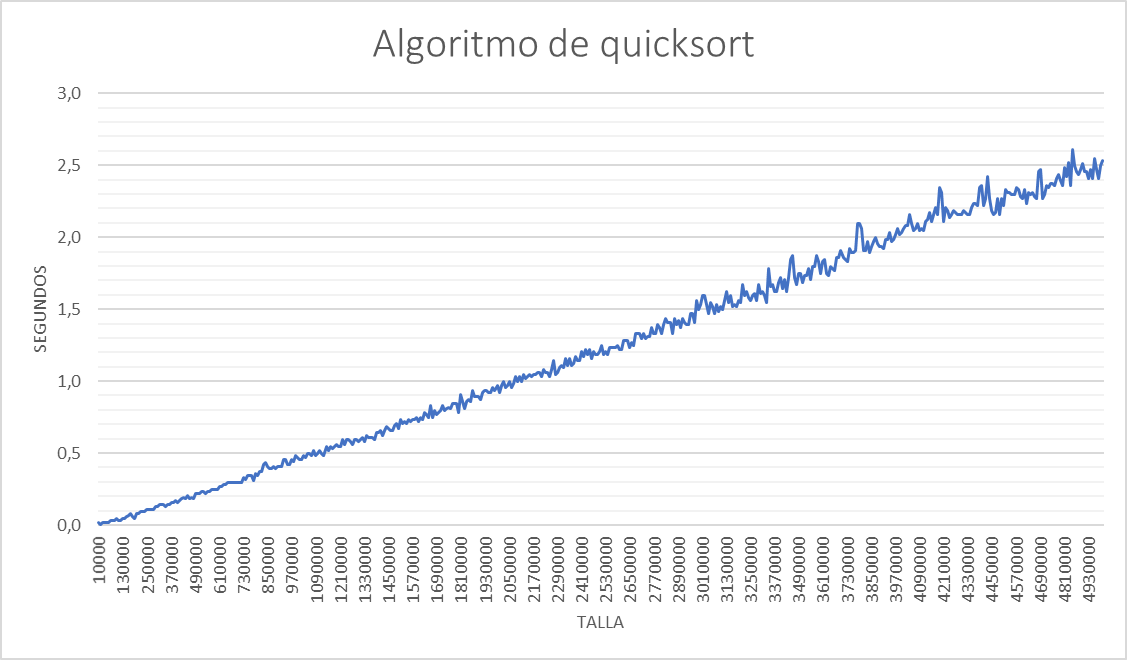
\includegraphics[scale=0.45]{../graficas/quicksort_sobremesa.png}
		\caption{Algoritmo de quicksort}
	\end{figure}

\newpage
\section{Algoritmo de burbulla}
	\paragraph{}
	Pártese dun tamaño inicial de 10.000 elementos, incrementando o vector en 10.000 e establécese como tamaño final un vector de 500.000 elementos, ao presentar unha orde promedia de $\Theta(n^{2})$.
	\paragraph{}
	Como se pode observar na figura 2, a gráfica presenta un aspecto cuadrático, na cal a ordenación inicial de 10.000 elementos tarda 0,421 segundos e a seguinte ordenación de 20.000 elementos tarda 1,672 segundos, ate un máximo de 1.091,563 segundos para 500.000 elementos.\\
	\begin{figure}[h]
		\centering
		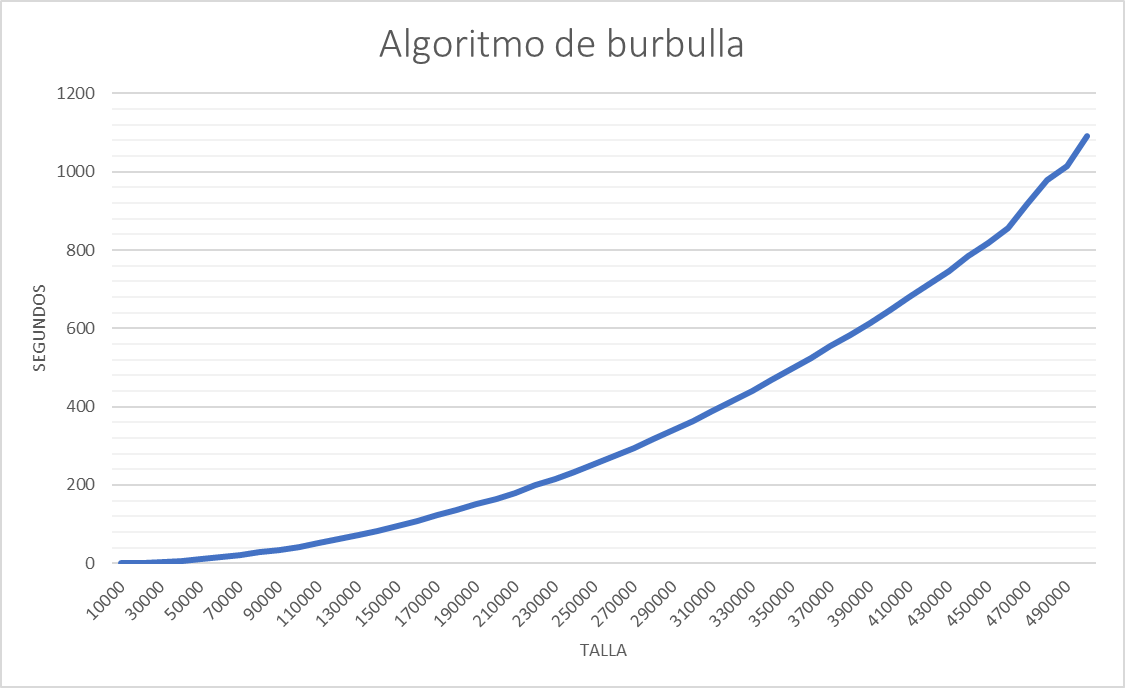
\includegraphics[scale=0.45]{../graficas/burbulla_sobremesa.png}
		\caption{Algoritmo de burbulla}
	\end{figure}
\newpage
\section{Algoritmo de selección}
	\paragraph{}
	Pártese dun tamaño inicial de 10.000 elementos, incrementando o vector en 10.000 e establécese como tamaño final un vector de 500.000 elementos, polos mesmos motivos que no apartado anterior.
	\paragraph{}
	Como se pode contemplar na figura 3, a gráfica presenta un aspecto cuadrático, máis pronunciado, na cal para a ordenación inicial de 10.000 elementos tarda 0,531 segundos e a seguinte ordenación de 20.000 elementos acádase en 2,14 segundos, ate un máximo de 1.287,109 segundos para o vector de 500.000 elementos.\\
	\begin{figure}[h]
		\centering
		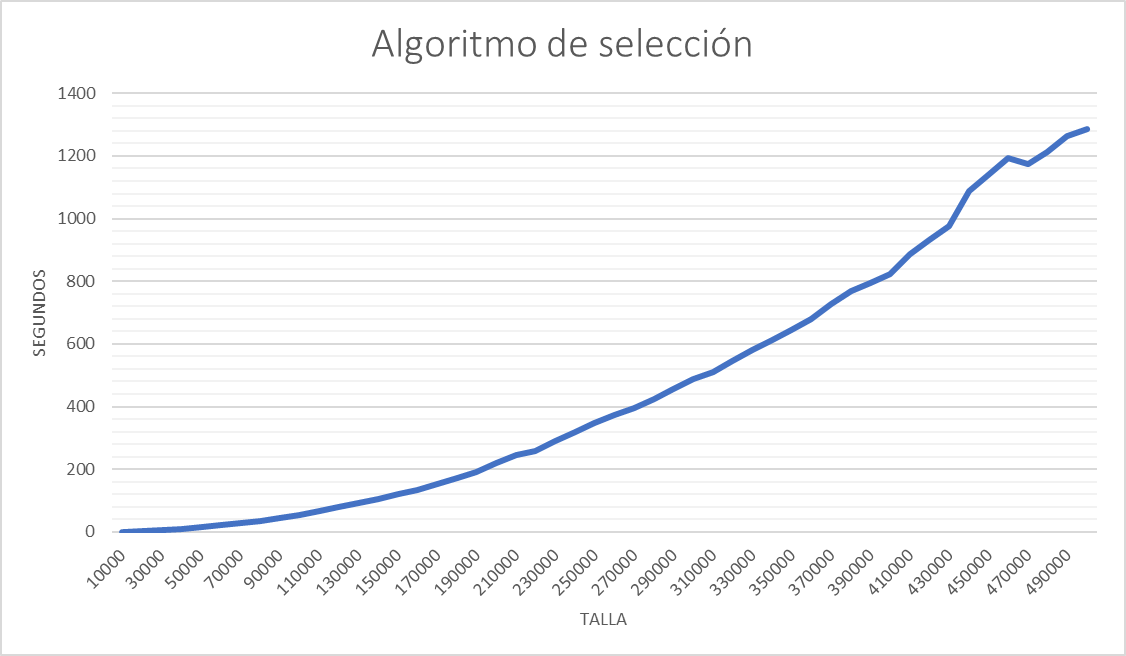
\includegraphics[scale=0.45]{../graficas/seleccion_sobremesa.png}
		\caption{Algoritmo de selección}
	\end{figure}

\newpage
\section{Conclusións}
	\paragraph{}
	Considerando como tempo razoable un intervalo de 10 segundos, o algoritmo de burbulla tardou 10,453 segundos manexando 50.000 elementos e o algoritmo de selección tardou 8,562 segundos para un tamaño de 40.000 elementos, mentras que o algoritmo de quicksort pode manexar vectores de 5 millóns de elementos en menos de 3 segundos (non se chegou a probar unha talla o suficientemente grande como para tardar 10 segundos).
	\paragraph{}
	En xeral, e especialmente para tallas grandes, o algoritmo de quicksort é moito máis rápido que os outros dous, podendo facer unha ordenación \textbf{dez veces maior en menos de 3 segundos}, mentras que tanto o de burbulla e selección tardan máis de 1.000 segundos para unha talla dez veces menor.
	\paragraph{}
	Tomando como tamaño de vector, o tamaño inicial de 10.000 elementos ou menos, poderíanse empregar indistintamente calquera dos tres algoritmos, posto que aínda que o quicksort tarde 0,016 segundos e os outros dous 0,421 e 0,531, ámbolos tres tardan menos dun segundo, tempo que se consideraría inapreciable.
	
\end{document}